\section{FOL formulation}
\begin{UnknownEnvironment}
	\color{red} Per motivare la non-necessarietà della caratterizzazione temporale per questo specifico problema, si vedano prima i punti A., B., C1 e C2. Infatti, possiamo esprimere tutte le caratteristiche temporali come dati associati agli eventi di traccia. Si veda $fol(\phi,c)$.
\end{UnknownEnvironment}
(Data) \emph{payloads} are finite functions $p\in V^K$, where $K$ is a finite set of keys and $V$ is a (finite) set of values. We distinguish the trace keys ($K_t$) from the event keys ($K_e$), such that $K=K_t\cup K_e$ with $K_t\cap K_e=\emptyset$. We denote $\bot$ as an element $\bot\notin V$: we can now denote $p(k)=\bot$ for $k\notin\textup{dom}(p)$.  An \emph{event} $e_j$ is a pair $\Braket{\const{a},p}\in \Activities\times V^K$, where $A$ is a finite set of activity labels and $p$ is a finite function describing the data payload. A \emph{trace} $\sigma$ is a ordered sequence of distinct events $e_1,\dots,e_n$ for which each event associates the same values to the same trace keys ($\forall \Braket{\const{a}_i,p_i},\Braket{\const{a}_j,p_j}\in \sigma.\forall k\in K_t. p_i(k)=p_j(k)$). A \emph{log} $\mathcal{L}$ is a finite set of {traces}, where each trace $\sigma$ is uniquely associated by a numeric case-id, $\textup{case}(\sigma)\in V$ . Last, we can freely assume that there exists a specific timestamp event key $T\in K_e$, such that for each trace $\Braket{\const{a}_1,p_1},\dots,\Braket{\const{a}_i,p_i},\dots,\Braket{\const{a}_n,p_n}$ it always exists
\begin{UnknownEnvironment}
	\color{red}A. Nel nostro contesto, assumiamo che non vi siano processi che avvengono contemporaneamente (non ci sono processi concorrenti), e che id di tracce differenti corrispondano a eventi che avvengono con una certa successione. Quindi, esiste sempre per ogni traccia del log una biiezione tra timestamp temporale e posizione dell'evento nella traccia. Sotto questa assunzione, possiamo esprimere il valore temporale dell'evento come si fa in ambito database, ovvero come un semplice valore dell'evento della traccia. 
	
	Vedi inoltre  Lemma 1 e 2.
\end{UnknownEnvironment}
 a bijection $i\overset{t}{\leftrightarrow} p_i(T)$, thus implying that temporal aspects of the events can be directly represented as payload values.

Values can represent either categorical data ($U^*$), numerical data ($F_{(\beta,t,\lambda,\omega)}$), 
\begin{UnknownEnvironment}
	\color{red} In \textit{Numerical Computing}, questo simbolo denota   l'insieme dei numeri reali rappresentabili finitamente (=in macchina) in base $\beta$, con $t$ cifre di mantissa e di esponenti tra $\lambda$ ed $\omega$. Sistematizzazione della notazione nel libro \textit{Numerical Linear Algebra}. 
\end{UnknownEnvironment}
or hierarchical data ($H$). Given $U$ the set of the UTF-32 characters, $U^*$ represents the set of all the possible strings, for which  a lexicographical ordering $\preceq_{U^*}$  exists. Numerical data can be represented via a finite number system $F_{(\beta,t,\lambda,\omega)}=\{\alpha\in\mathbb{R}|\alpha=\pm (\sum_{i=0}^{t-1}\alpha_i\beta^i)\beta^p,\;\lambda\leq p\leq \omega\}\cup\Set{0}$, where IEEE floats are represented by $F_{(2,23,-126,127)}$, for which it trivially exists an ordering $\preceq_{\mathbb{R}}$. Hierarchical data can be described as a partially ordered set $(H,\preceq_H)$, where $\preceq_H$ determines an is-a relationship among entities. Please note that is always possible to compose multiple hierarchies into one single hierarchy via graph cartesian product \cite{BergamiBM20}. 

At this point, we want to prove that each log $\mathcal{L}$ can be described as a finite model: 
\begin{UnknownEnvironment}
	\color{red} B. Assunzione (1): vogliamo effettuare l'allineamento della traccia $\sigma$ con un insieme di clausole $\mathcal{M}$. Per definizione $\sigma\vDash\mathcal{M} \Leftrightarrow \sigma\in L[\mathcal{M}]$. La distanza di allinamento zero mi identifica quindi la soddisfacibilità: quindi, la distanza di allineamento può essere utilizzata per fornire una nozione di soddisfacibilità approssimata per il problema Max-SAT. 
	
	Assunzione (2): dato lo use case nella precedente assunzione, lavoriamo con un Close World Assumption, dove  $\mathcal{M}$ è soddisfacibile se esiste almeno una traccia $\sigma$ del log $\mathcal{L}$ che soddisfa $\mathcal{M}$. Altrimenti, diremo che $\mathcal{M}$ non è mai soddisfatto in $\mathcal{L}$. Quindi, $\mathcal{L}\vDash\mathcal{M}\Leftrightarrow\exists \sigma\in\mathcal{L}. \sigma\vDash\mathcal{M}$.
	
	Caso diverso è per i SAT-solvers \cite{LiPZVR20}, dove $\mathcal{L}$ non è dato e quindi la decisione se una formula è soddisfacibile prescinde dalla generazione di un witness di soddisfacibilità, che non è nota a priori. In quel caso, non possiamo fare a meno che ``attendere'' finché non si trova un esempio o un controesempio.
\end{UnknownEnvironment}

this is a sufficient requirement to make any FOL formula decidable \cite{harrop},
\begin{UnknownEnvironment}
	\color{red} C1. Il libro di testo dal quale ho tratto questa possibilità, cita l'articolo di Harrop. \textit{For syntactically restricted classes of formulas, it often turns out that satisfiability, i.e. having a model at all, is equivalent to having a finite model. (Or dually, validity is equivalent to holding in all finite models).}  Nel nostro caso, effettuiamo una restrizione sintattica su tutte le possibili proposizioni che possiamo ottenere dal log $\mathcal{L}$. 
	
	Si veda Lemma 1.
\end{UnknownEnvironment} as we just need to enumerate larger and larger finite interpretations of a given trace until we find one in which it holds.
\begin{UnknownEnvironment}
	\color{red} C2. Sempre dallo stesso libro summenzionato, questo segue dal seguente teorema: \textit{There is a systematic procedure for deciding the validity (satisfiability) of all formulas with the finite model property for validity (resp. satisfiability)}. Questo è mostrato nel libro anche tramite del codice OCaml dove, se abbiamo un modello finito di interpretazioni di dimensioni finite, è sempre possibile enumerare tutte le possibili interpretazioni finite del suddetto modello. Questo è il nostro caso, perché il log è finito, ed ogni singola traccia è finita. Quindi, possiamo scandire ogni singola traccia in tempo finito, in quanto dal nostro insieme finito non definiamo mai un'interpretazione infinita, potenzialmente semidecidibile.
\end{UnknownEnvironment}
\begin{UnknownEnvironment}
{\color{blue} Nel nostro caso quindi, siamo interessati a verificare la soddisfacibilità di un modello $\mathcal{M}$ all'interno di un insieme di tracce nel log $\mathcal{L}$. Quindi, l'insieme di tutti i valori possibili è finito. Dato che su ciascuno di questi domini dei valori è definibile una relazione d'ordine, possiamo definire una relazione d'ordine $\preceq_V$, ed enumerare tutte le possibili combinazioni di valori che soddisfano $\preceq_V$. Osserva inoltre che, tra questi valori, saranno presenti anche i valori temporali, rappresentati numericamente. Sposto questo lemma qui, precedentemente nell'appendice.}
\end{UnknownEnvironment}
\begin{lemma}\label{lem:hu}
	Values can be represented as a finite partially ordered set $\mathcal{V}=(V\cup\{\top,\bot\},\preceq_V)$.
\end{lemma}
\begin{proof}
	Values in $V$ can be described by either categorical data, numerical data, or hierarchical data. For categorical data in $U^*$, it always exists a trivial lexicographical ordering $\preceq_{U^*}$. Given that finite number systems represent a finite set of real numbers in $\mathbb{R}$, numerical data expressed as such always admits the same ordering as the real numbers, which are a poset $(\mathbb{R},\preceq_{\mathbb{R}})$. Last, given that hierarchical data can be expressed as DAGs $(H,\preceq_H)$, where $H$ are the hierarchy's entities and $\preceq_H$ expresses the is-a relationships, $(H,\preceq_H)$ is a poset \cite{BergamiBM20}. Given that $U^*$, $H$, and $F_{(2,23,-126,127)}$ are sets of distinct elements, we can represent $V$ as a finite set of values completely describing the payloads of a log $\mathcal{L}$ as follows:
	\[V=\bigcup_{e_i\in \mathcal{L}}\Set{p(K)|\Braket{\const{a}, p}\in e_i}\backslash\{\bot\}\]
	After defining $\bot$ as the minimal element of $V$ and $\top$ the maximal element of such set, we can define an ordering $\preceq_V$ as follows:
	\begin{align*}
	\forall u,v\in V.\; &u\preceq_V v\Leftrightarrow &&\;(u\in U^*\wedge v\in U^*\wedge u\preceq_{U^*}v)\\
	& &&\vee (u\in F_{(\beta,t,\lambda,\omega)}\wedge v\in F_{(\beta,t,\lambda,\omega)}\wedge u\preceq_{\mathbb{R}}v)\\
	& &&\vee (u\in H v\in H\wedge u\preceq_{H}v)\\
\forall s\in\min(U^*\cap V).\;&\bot\preceq_V  s\\
	\forall s\in\max(U^*\cap V).\;&s\preceq_V  \top\\
	\forall f\in\min(F_{(2,23,-126,127)}\cap V).\; &\bot\preceq_V f \\
	\forall f\in\max(F_{(2,23,-126,127)}\cap V).\; &f\preceq_V \top \\
	 \forall h\in \min(H\cap V).\;&\bot\preceq_V  h\\
	 \forall h\in \max(H\cap V).\;&h\preceq_V  \top\\
	\end{align*}
\end{proof}



\begin{lemma}
	Each log $\mathcal{L}$ can be represented as a finite model $\color{blue}\Delta(\mathcal{L})$.
\end{lemma}
\begin{proof}
	Let  $A\cup\{\mathtt{``}{\preceq_V}\mathtt{"}\}$ be the set of the predicate symbols. Each predicate symbol $\const{a}\in A$ represents an $(|K|+1)$-ary predicate, while $\mathtt{``}{\preceq_V}\mathtt{"}$ represents a binary predicate. Given that Lemma \ref{lem:hu} completely characterizes the Herbrand's Universe $U(\mathcal{L})=\mathcal{S}$ for the finite log $\mathcal{L}$ as a finite set and given that the set of symbols is also finite, the resulting Herbrand's Base $B(\mathcal{L})$ for the log $\mathcal{L}$ is also a finite set of grounded atoms. Given that any possible Herbrand model resulting from such base is finite, then the set of all the possible {\color{blue}worlds} is finite, and each {\color{blue}world} is finite. Therefore, the resulting model $\color{blue}\Delta(\mathcal{L})$ is finite.
	
	
	Each $i$-th event $\Braket{\const{a}_i,p_i}$ from a trace $\sigma\in\mathcal{L}$ can be represented for $K=\Set{T,k_2,\dots,k_n}$ as a $(n+1)$-ary predicate $\const{a}_i(\textup{case}(\sigma),i,p_i(k_2),\dots,p_i(k_n))$. Therefore, $\mathcal{L}$ can be represented as follows:
	\begin{align*}
	\Delta(\mathcal{L})=&\Set{\mathtt{``}{\preceq_V}\mathtt{"}(u,v)|u,v\in B(\mathcal{L})\wedge u\preceq_V v}\cup\\
	&\Set{\const{a}_i(\textup{case}(\sigma),i,p_i(k_2),\dots,p_i(k_n))|\Braket{\const{a}_i,p_i}\in e_i,e_i\in\mathcal{L}}
	\end{align*}
\end{proof}

Walking on the footsteps of \cite{GiacomoMM14}, we can provide a semantics to the LTL$_f$ formulae over the previously given Herbrand Base $\Delta(\mathcal{L})$. We can {\color{blue}interpret} an LTL$_f$ formula {\color{blue}in negation normal form} as $\textit{fol}(\phi,\textup{case}(\sigma))$ for each trace $\sigma$
\begin{UnknownEnvironment}
	\color{red}Osserva: la semantica delle formule LTL$_f$ è definito su ogni singola traccia. Quindi, non sono possibili template Declare che definiscano le intere proprietà del log, come il numero delle tracce del Log.
\end{UnknownEnvironment}
as follows:
\[\textit{fol}(\phi,c)=\begin{cases}
\exists x_1,\dots,x_m\in \mathcal{S}. \textit{pl}(\phi,c,{\color{magenta}1}) & \Set{x_1,\dots,x_m}=\textit{FV}(\textit{pl}(\phi,c,{\color{magenta}1}))\\
\textit{pl}(\phi,c,{\color{magenta}1}) & \textup{oth.}\\
\end{cases}\]
{\color{blue}where \textit{pl} is inductively defined over $\phi$ as follows:}
\[\textit{pl}(\phi,c,{\color{magenta}t})=\begin{cases}
\const{a}(c,{\color{magenta}t},\actsymb{({x_{\const{a}\mathbf{P}}})}{\color{black}2}[\color{magenta}t],\dots,\actsymb{({x_{\const{a}\mathbf{P}}})}{n}[\color{magenta}t])\wedge \mathbf{P}  &\phi=\const{a}\wedge \mathbf{P}\\

\neg \textit{pl}(\phi,c,{\color{magenta}t}) & \phi=\neg \phi\\
\textit{pl}(\phi,c,{\color{magenta}t+1}) & \phi=\Next \phi\\	 
\bigvee_{\color{magenta}t\leq\tau\leq|\sigma|}\textit{pl}(\phi,c,{\color{magenta}\tau}) & \phi=\lozenge\phi\\
\bigwedge_{\color{magenta}t\leq\tau\leq|\sigma|}\textit{pl}(\phi,c,{\color{magenta}\tau}) & \phi=\square\phi\\
\textit{pl}(\phi_1,c,{\color{magenta}t})\wedge \textit{pl}(\phi_2,c,{\color{magenta}t}) & \phi= \phi_1\wedge \phi_2\\
\textit{pl}(\phi_1,c,{\color{magenta}t})\vee \textit{pl}(\phi_2,c,{\color{magenta}t}) & \phi= \phi_1\vee \phi_2\\
\bigvee_{\color{magenta}t\leq\tau\leq|\sigma|}\textit{pl}(\phi_2,c,{\color{magenta}\tau})\wedge\bigwedge_{\color{magenta}t\leq u<\tau}\textit{pl}(\phi_1,c,{\color{magenta}u}) & \phi= \phi_1\Until \phi_2\\

\bigwedge_{\color{magenta}t\leq\tau\leq|\sigma|}\textit{pl}(\phi_2,c,{\color{magenta}\tau})\vee\bigvee_{\color{magenta}t\leq u<\tau}\textit{pl}(\phi_1,c,{\color{magenta}u}) & \phi= \phi_1\Release \phi_2\\
{\color{blue}\dots} & {\color{blue}\dots} \\

%\textit{pl}(\neg\lozenge\neg \phi,c,t) & \phi=\square\phi\\
\end{cases}\] 
\begin{UnknownEnvironment}
	\color{magenta}Ora, lo scopo di questa formalizzazione non è tanto quello di fornire una formalizzazione elegante dove la FOL contempla separatamente il tempo, quanto quello di mostrare come la soddisfacibilità di una formula per una traccia è computabile eseguendo un algoritmo decidibile, in quanto anche il dato temporale è esprimibile tramite valori sul poset $\mathcal{S}$. Nella versione finale del paper, possiamo ragionare su come rappresentare sintatticamente in modo elegante questa logica. 
\end{UnknownEnvironment}
%\[\textit{pl}(\lozenge\phi,c,t)=\textit{pl}(\mathbf{True}\Until \phi,c,t)=\mu_{t\leq\tau\leq|\sigma|}\textit{pl}(\phi,c,\tau)\]
%
%\[\textit{pl}(\square\phi,c,t)=\neg\mu_{t\leq\tau\leq|\sigma|}\textit{pl}(\neg\phi,c,\tau)\]

%\begin{align*}
%F_t(\phi_1\Until \phi_2)&=F_t(\phi_2)\vee \left(F_t(\phi_1)\wedge F_{t+1}(\phi_1\Until \phi_2)\right)\\
%	&=F_t(\phi_2)\vee \left(F_t(\phi_1)\wedge \left(F_{t+1}(\phi_2)\vee \left(F_{t+1}(\phi_1)\wedge F_{t+2}(\phi_1\Until \phi_2)\right)\right)\right)\\
%	&=F_t(\phi_2)\vee \left(\left(F_t(\phi_1)\wedge F_{t+1}(\phi_2)\right)\vee \left(F_t(\phi_1)\wedge F_{t+1}(\phi_1)\wedge F_{t+2}(\phi_1\Until \phi_2)\right)\right)\\
%\end{align*}
%
%Traditionally, $\textit{pl}(\phi_1\Until \phi_2,c,t):=\textit{pl}(\phi_2,c,t)\vee \left(\textit{pl}(\phi_1,c,t)\wedge \textit{pl}(\phi_1\Until \phi_2,c,t+1)\right)$. Given that each trace $\sigma$ having $\textup{case}(\sigma)=c$ is finite, we can finitely represent such predicate as follows:
%\[\textit{pl}(\phi_1\Until \phi_2,c,t):=\bigvee_{t\leq \tau\leq |\sigma|}\left(\textit{pl}(\phi_2,c,\tau)\wedge\;\bigwedge_{t\leq u<\tau}\textit{pl}(\phi_1,c,u)\right)\]
%The latter formula means that either $\textit{pl}(\phi_1,c,\tau)$ always holds from $t$ until the end of the trace ($t\leq \tau\leq |\sigma|$), or it exists at least one single instant $t<\tau\leq|\sigma|$ for which $\textit{pl}(\phi_2,c,\tau)$ holds while $\textit{pl}(\phi_1,c,u)$ holds for all the remaining times $t\leq u<\tau$. 
where each predicate $\mathbf{P}$ is a relation predicate that can be expressed in terms of $\mathtt{``}\preceq_V\mathtt{"}$. Please observe that, differently from \cite{DBLP:conf/bpm/MaggiDGM13} the existential quantification over the payload values was pulled at the beginning of the formula as in the tuple relational calculus \cite{10.1145/362384.362685}  to guarantee the expression of join conditions. E.g.,:
{\color{blue} Questo invece mi serve per poter esprimere tutti i predicati che possiamo esprimere in modo Declare Data Aware tramite la summenzionata relazione d'ordine $\preceq_V$.}
\begin{itemize}
	\item given a constant value $\kappa$, the condition $\textit{Cond}:=\const{a}_i.K_j\preceq_V \kappa$ to be tested at time $t$ can be expressed as $\mathbf{P}:=(x_{\const{a}_i\textit{Cond}})_j^t\preceq_V\kappa$
	\item the join condition $\textit{Join}:=\const{a}_i.K_j\preceq_V \const{a}_h.K_k$ where $\const{a}_i$ happening at time $t$ {\color{blue}temporally} follows $\const{a}_j$  can be expressed as $\mathbf{P}:=\bigvee_{\tau<t,\textit{Cond}}(x_{\const{a}_i\textit{Join}})_j^t\preceq_V (x_{\const{a}_h\textit{Cond}})_k^\tau$
\end{itemize} 


%$\sigma$ is a {\color{blue}possible world} for $\phi$ iff. $\Delta(\{\sigma\})\vDash\textit{pl}(\phi,\textup{case}(\sigma),1)$. Consequently, a log $\mathcal{L}$ is a {\color{blue}finite} model for $\phi$ if all of its traces are {\color{blue}possible worlds} for $\phi$. 
{\color{blue}A Declare Data Aware model $\mathcal{M}$ is a set of instantiated Declare Data Aware templates $\mathcal{M}=\Set{C_i}_{i\leq n}$, where each template $C_i$ can be expressed in LTL$_f$ via a translation function $\translation{\textup{D}}{\textup{LTL}_f}$, such that $\translation{\textup{D}}{\textup{LTL}_f}(C_i)$ is a well-formed LTL$_f$ formula. The usual semantic interpretation of such model $\mathcal{M}$ is the conjunction of all of such interpretations, and therefore $\sem{\mathcal{M}}=\bigwedge_{C_i\in\mathcal{M}}\translation{\textup{D}}{\textup{LTL}_f}(C_i)$. Therefore, the satisfiability of a log trace $\sigma\in\mathcal{L}$ can be expressed as $\sigma\vDash\mathcal{M}\Leftrightarrow \bigwedge_{C_i\in\mathcal{M}}\textit{fol}\left(\translation{\textup{D}}{\textup{LTL}_f}(C_i),\;\textup{case}(\sigma)\right)$.}
\begin{UnknownEnvironment}
	\color{red} Si veda l'ultima equazione a pagina 13 e spiegazione associata su come esprimere la congiunzione tramite intersezione.
\end{UnknownEnvironment}
After observing that the only instance of the existential quantifier is merely a way to bound the payload values to a predicate via variables $({x_{\const{a}\mathbf{P}}})_2^t,\dots,({x_{\const{a}\mathbf{P}}})_k^t$, and given that at each timestamp $t$ only one event can occur in a trace with case-id $c$
\begin{UnknownEnvironment}
	\color{red} (in virtù della possibilità di effettuare la biiezione tra timestamp ed id di evento nella traccia, e poiché tutte le tracce del log sono finite, ed il log è finito, \dots)
\end{UnknownEnvironment}
, then the former FOL fragment is decidable via quantifier elimination. 
\begin{UnknownEnvironment}
	\color{red} (poiché per ogni traccia con case-id $c$ esisterà un unico evento che avviene in un determinato istante temporale, e quindi posso ottenere quali sono i dati ad essi associati \dots)
\end{UnknownEnvironment}In particular, the former definition implies that the it is always possible to test whether a trace $\sigma$ is a {\color{blue}possible world} for a given Data Aware Declare template $\phi$ in polynomial time over the size of the trace and in exponential time over the query size, similarly to SQL queries \cite{DBLP:conf/stoc/Vardi82}. 
\begin{UnknownEnvironment}
	\color{red} Dato che anche l'algoritmo in \S\ref{ref:agm} così la soluzione \S\ref{ref:dddmm} per il momento accantonata hanno la stessa complessità computazionale dell'interpretazione della formula, idealmente questi algoritmi sono plausibili. Manca una dimostrazione formale.
\end{UnknownEnvironment}



\section{Alternative approaches to approximate Data Aware Declare Model Matching}
\subsection*{Preliminary Notation}
The alignment $\gamma_{\sigma,\sigma'}$ denotes the optimal alignment for $\sigma$ over $\sigma'$ having an alignment cost of $\mathcal{K}(\gamma_{\sigma,\sigma'})$. 
\subsection{Baseline}


\begin{table}[!t]
	\centering
	\begin{tabular}{c|c}
		\toprule
		Declare Constraints & LTL$_f$ semantics\\
		\midrule
		$\mathsf{CoExistence}(\textit{LIC},\textit{LMH})$ & $(\lozenge\textit{LIC}\Rightarrow\lozenge\textit{LMH})\wedge (\lozenge\textit{LMH}\Rightarrow \lozenge\textit{LIC})$  \\
		
		$\mathsf{Precedence}(\textit{SQ},\textit{RQR})$ & $\neg \textit{RQR}\; \mathcal{W}\; \textit{SQ}\qquad \equiv \qquad (\neg \textit{RQR}\; \Until\; \textit{SQ})\vee \square\textit{RQR} $  \\
		\bottomrule
	\end{tabular}
\caption{Some Declare constraints \cite{LeoniMA12}}
\end{table}



\begin{figure}[!t]
	\centering
	\subfloat[][$\mathsf{CoExistence}(\textit{LIC},\textit{LMH})$]{\includegraphics[width=.5\textwidth]{images/m1.png}\label{fig:m1}}\quad
	\subfloat[][$\mathsf{Precedence}(\textit{SQ},\textit{RQR})$]{\includegraphics[width=.3\textwidth]{images/m2.png}\label{fig:m2}}\quad
	\caption{Automata generated for Declare templates using \cite{LeoniMA12,DBLP:conf/bpm/Westergaard11}}\label{fig:ma}
\end{figure}

\subsection{A$^*$ space search}
Given a Declare model $\mathcal{D}=(\Activities,\Pi)$, where $\Pi$ is a set of Declare constraints $\pi_i$ which semantics can be represented as a LTL$_f$ formula $\phi_i$ \cite{GiacomoMM14}. Each of these formulae can be represented as a single DFA$_{\phi_i}$ \cite{LeoniMA12}  using one of the algorithms proposed in \cite{DBLP:conf/bpm/Westergaard11}; these graphs are edge labelled by a set of non-negated activity labels (Figure~\ref{fig:ma}). Furthermore, a trace is valid for $\sigma\in L(\mathcal{D})$ if it is accepted by all the generated automata, i.e., $\sigma\in L(\mathcal{D})\Leftrightarrow\sigma\vDash\mathcal{D}\Leftrightarrow \forall \pi_i\in\Pi. \sigma\in L(\textup{DFA}_i) $; as a result, a model trace is the set of all the valid model traces generated by all the automata.

An alignment of a trace $\sigma$ with a declare model $\mathcal{D}$ is performed via a A* search algorithm, starting from an empty alignment $\gamma_\emptyset$. The computation halts when we reach an alignment $\gamma_{\sigma,\sigma_M}$ where $\sigma_M\in L(\mathcal{D})$. As the number of the model traces  $|L(\mathcal{D})|$  is potentially a countably infinite set, the graph for the A* is not completely constructed before running the algorithm, while it is generated while visiting the candidate neighbor nodes of the currently visited node. Given a currently visited node $\gamma_{\sigma,\varsigma}$, we could possibly move to a neighbour node $\gamma_{\sigma c,\varsigma d}$ where $(c,d)$ is a valid move. The candidate node to be visited after $\gamma_{\sigma,\varsigma}$ is elected among the nodes within a priority queue having the minimum evaluation function $f(\gamma_{\sigma,\varsigma})=g(\gamma_{\sigma,\varsigma})+h(\gamma_{\sigma,\varsigma})$, where such functions are defined as follows:
\begin{itemize}
	\item $g(\gamma_{\sigma,\varsigma})=\kappa^{\min}|\varsigma|+\mathcal{K}(\gamma_{\sigma,\varsigma})$
	\item $h(\gamma_{\sigma,\varsigma})=\underset{\sigma_M\in L (\mathcal{D}),\varsigma\subseteq\sigma_M }{\min}\kappa^{\min}(|\sigma_M|-|\varsigma|)$
\end{itemize}
In order to reduce the number of comparisons between all the automata associated to the declare model, we can potentially generate one single automaton out of the  by performing the kronecker product among all the DFA$_i$-s \cite{DBLP:conf/edbt/BergamiMM17} where we preserve the edges having no empty intersection in their labels: given two DFAs $G_1=(V_1,E_1,s_1,F_1)$ and $G_2=(V_2,E_2,s_2,F_2)$, the product DFA is $G_1\times G_2=(V_1\times V_2, E_\times,s_1\times s_2,F_1\times F_2)$, where: $E_\times = \{((a,c),(b,d))\in (V_1\times V_2)^2|(a,b)\in E_1,(c,d)\in E_2,\lambda(a,b)\cap\lambda(c,d)\neq\emptyset\}$. As a result, we do not require 
\checkmark for describing trace alignments while we can exploit string matching scoring functions \cite{CAiSE21}. The resulting graph product preserves the alignment equivalence requirements in \cite{LeoniMA12}, where further space reduction strategies are also described. 

This approach can be extended to handle Data Aware Declare models by defining $\Sigma=\Activities\cup \Activities\cdot\{\mathbf{P}_1,\dots,\mathbf{P}_n\}$, where $\{\mathbf{P}_1,\dots,\mathbf{P}_n\}$ is the set of the Data Aware Declare predicates appearing within the model of interest, and by eploiting the following cost function:
\[\kappa(a_1,a_2)=\begin{cases}
	\delta_a(a_1, \const{a}) &  a_2=\const{a}\mathbf{P} \wedge \mathbf{P}(a_1)\\
	\delta_b(a_1, \const{a}) &  a_2=\const{a}\mathbf{P} \wedge \neg\mathbf{P}(a_1)\\
	\delta_c(a_1,\const{a}) & a_2=\const{a} \\
\end{cases}\]
where $\delta_a$, $\delta_b$, and $\delta_c$ are cost functions among strings over three different scenarios. 

\begin{figure}[!t]
	\centering
	\subfloat[][$\mathsf{CoExistence}(\textit{LIC},\textit{LMH})$]{\includegraphics[width=.5\textwidth]{images/g1.png}\label{fig:vm1}}\quad
	\subfloat[][$\mathsf{Precedence}(\textit{SQ},\textit{RQR})$]{\includegraphics[width=.45\textwidth]{images/g2.png}\label{fig:vm2}}\quad
	%\subfloat[][$\square((\const{a}\wedge \mathbf{P}_1)\Leftrightarrow \lozenge(\neg\const{b}\wedge \neg\mathbf{P}_2))$]{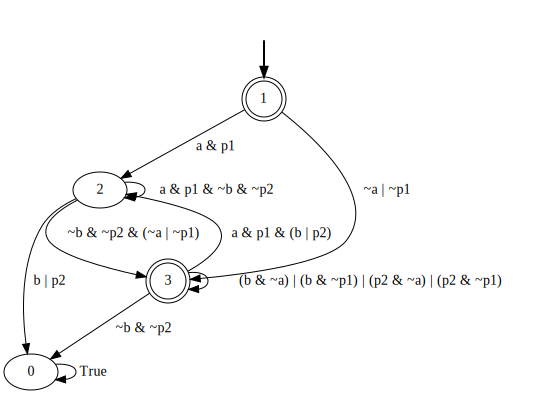
\includegraphics[width=.5\textwidth]{images/img3.png}\label{<figure3>}}
	\caption{Automata generated for Declare templates using \cite{GiacomoV13,GiacomoMM14}}\label{fig:mma1}
\end{figure}
\begin{figure}
	\centering
	\includegraphics[width=\textheight,angle=90]{images/g3.png}\caption{Automata for $\mathsf{CoExistence}(\textit{LIC},\textit{LMH})\wedge\mathsf{Precedence}(\textit{SQ},\textit{RQR})$ generated using using \cite{GiacomoV13,GiacomoMM14}}\label{fig:mma2}\quad
\end{figure}
\subsection{Approximate Graph Matching}\label{ref:agm}
Given that the previous approach requires an heuristic for determining the best alignment of a trace, we want to identify an algorithm providing the best alignment in polynomial time, without necessarily pruning a potentially infinite search space and by exploiting no heuristic functions. 

The semantics of Declare models can be expressed as a single LTL$_f$ formula $\phi$: in particular, we can represent each of these  as a single NFA$\phi$, such that $\sigma\vDash\phi\Leftrightarrow \sigma\in L(\textup{NFA}_\phi)$ \cite{GiacomoV13,GiacomoMM14}, where $L(\textup{NFA}_\phi)$ is the language generated by $\textup{NFA}_\phi$ (Figure~\ref{fig:mma1} and \ref{fig:mma2}). Given a set of atomic tasks $\Activities$, $\textup{NFA}_\phi$ is a graph, where  the nodes represent the formulae that are valid for all the traces that are accepted starting from this node, and  edges are labelled with  a combination of predicates $\mathcal{P}=\Activities$ in disjunctive normal form: edges can be traversed only if the currently-visited event satisfies the associated condition. This problem formulation does not allow to perform trace alignments, as the testing condition is a boolean condition. 


On the other hand, it is always possible to approximately align a trace $\sigma$ to a node-labelled automaton $N$ having one single accepting (and initial) state \cite{Myers1989}. Given that it is always possible to transform a $\textup{NFA}_\phi$ to a node-labelled graph \cite{CAiSE21} as required by \cite{Myers1989}, the algorithm starts by transforming a trace $\sigma$ to a node-labelled path $P_{\tau\sigma}$; given $N$, it generates a novel automaton $P_\sigma\square N$, which initial (accepting) state is the node-pair representing the initial (accepting) states for both automata, and $\square$ is the graph cartesian product \cite{10.5555/2031398}. Next, we annotate each edge as either a deletion, an insertion, a substitution, or a null (no mis-alignment) edge with possibly arbitrary alignment costs: as a result, all the paths between the initial state and the final state of $P_\sigma\square N$ represent all the possible alignments between $\sigma$ and the sequences of $L(A_\phi)$, and the shortest path models the minimum alignment. Please observe that, by construction, a minimum-weight path may be found by considering only those paths that are cycle free \cite{10.5555/2031398}. Consequently, this problem reduction proves that the alignment of a trace against a declare model can be performed in polynomial time over the size of the data and in exponential time over the size of the query, similarly to the query semantics of SQL queries \cite{DBLP:conf/stoc/Vardi82}.

Albeit NFAs generated in \cite{GiacomoV13,GiacomoMM14} mainly refer to usual Declare models, such solution can be also extended to Data Aware Declare models by extending $\mathcal{P}$ with the data predicates $\{\mathbf{P}_1,\dots,\mathbf{P}_n\}$ within the Data Aware Delcare model of interest.

Please observe that this solution limits the expressivity of the nodes predicates to conditions $\mathbf{P}_i$ that can be only verified over one single event. In fact, the predicates associated to each edge can be only tested over the event currently accessed while visiting the automata, as NFAs have neither registers nor stacks to remember a payload coming from a previously accepted event. Consequently, join conditions among events cannot be expressed \cite{SchonigCMM16}. \texttt{\color{red}[TODO: can we possibly represent join conditions among traces' events by changing the way\\ for which the NFA is generated from LTL$_f$? Does the representation\\ of join conditions necessarily requires Büchi automata?]} For this reason, we propose a data-driven solution, where join condition can be naturally expressed.


%Domanda: il tool \url{https://flloat.herokuapp.com/} ha generato il seguente automa per 


